\section{Ejercicio 7}

Bajo la métrica tiempo de respuesta (esto es, el tiempo que tarda desde que se genera un pedido hasta que se obtiene la respuesta) esperamos que el quantum óptimo sea el menor posible, ya que a esta métrica solo concierne la cantidad de tiempo que pasa desde el pedido hasta la atención de la tarea, y con un quantum mayor, se es`era que cada tarea deba esperar mas tiempo hasta ser atendida, ya que debe esperar a que las tareas que están corriendo terminen su quantum. 


Sin embargo, al tener un quantum mas grande, se pierde menos tiempo realizando cambios de contexto, siguiendo este razonamiento, un quantum alto debería tener un mejor puntare en una medida que tenga que ver con la velocidad de ejecución de las tareas.

Es así que proponemos como segunda medida el THROUGHPUT (cantidad de procesos que terminan por unidad de tiempo). En este caso se espera como se comento anteriormente un desempeño superior de un quantum mas alto.


Presentamos 4 instancias de cuatro tareas TaskBatch con 3 bloqueos para todas las tareas. Los gráficos resultantes son los siguientes y los usamos como base para las conclusiones más abajo.


\begin{figure}[H]
  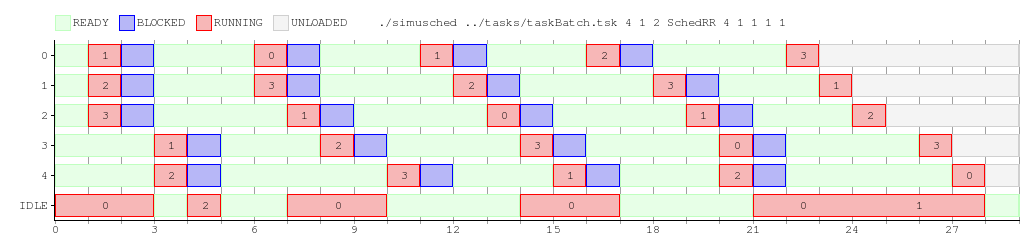
\includegraphics[width=\textwidth]{ej7/salida.png}
  \caption{Tarea con 1 quantum.}
\end{figure}

\begin{figure}[H]
  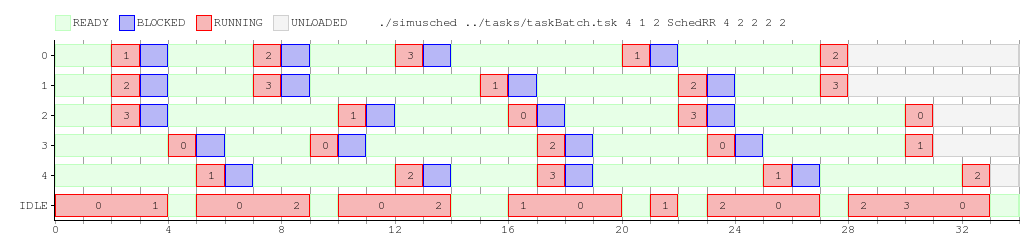
\includegraphics[width=\textwidth]{ej7/salida2.png}
  \caption{Tarea con 2 quantums.}
\end{figure}

\begin{figure}[H]
  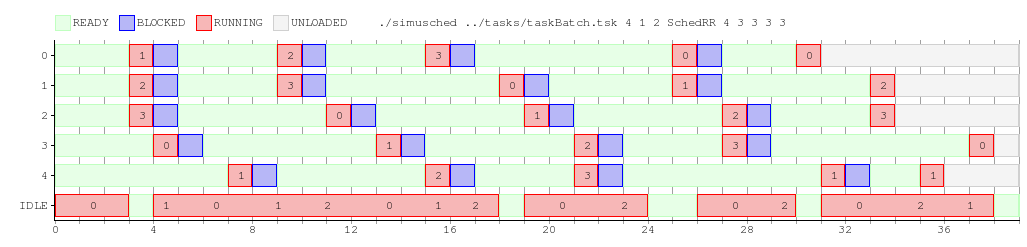
\includegraphics[width=\textwidth]{ej7/salida3.png}
  \caption{Tarea con 3 quantums.}
\end{figure}

\begin{figure}[H]
  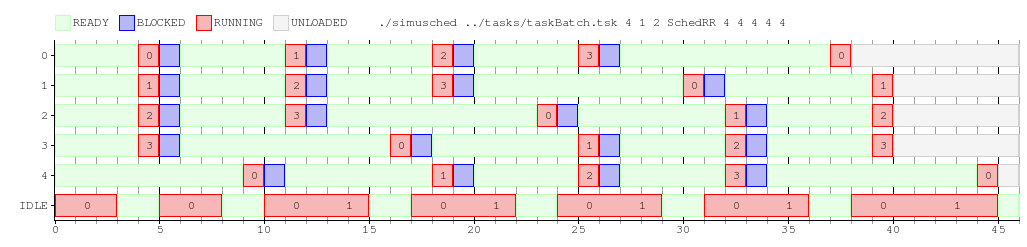
\includegraphics[width=\textwidth]{ej7/salida4.png}
  \caption{Tarea con 3 quantums.}
\end{figure}


Como se puede observar en la experimentación realizada el quantum mas chico fue el que mejor resultados dio en cuanto al tiempo de respuesta.

